\documentclass[aps,prl,reprint,amsmath,amssymb,floatfix,nofootinbib]{revtex4-2}
\usepackage{graphicx}
\usepackage{orcidlink}
\usepackage{bm}
\usepackage{hyperref}

% -------------- Margin Stamp ----------------
\usepackage[style=iso]{datetime2}
\usepackage{FiraMono}
\usepackage{tikz}

\AddToHook{shipout/background}{
  \begin{tikzpicture}[remember picture, overlay]
    \node [rotate=-90, color=gray!80, font=\fontfamily{FiraMono-TLF}\selectfont\footnotesize] at ([xshift=-1.2cm]current page.east) {WORKING DRAFT \quad 
    $\bullet$ \quad \DTMnow \quad 
    $\bullet$ \quad \href{https://doi.org/10.5281/zenodo.20279094}{doi.org/10.5281/zenodo.20279094} \quad 
    $\bullet$ \quad Brian S. Mulloy \quad 
    $\bullet$ \quad bmulloy@umich.edu};
  \end{tikzpicture}
}
% --------------------------------------------------------

\begin{document}

\title{Wigner Resolution from Action Capacity}

\author{Brian S. Mulloy\orcidlink{0000-0002-1803-3172}}
\affiliation{Independent Researcher, Corktown, Detroit, Michigan, USA}
\email{bmulloy@umich.edu}

\date{\today}

\begin{abstract}
The Wigner function represents a quantum state in phase space. Smoothing it gives a non-negative portrait, with the smoothing scale conventionally set from outside the state. We show that the scale is set by the state. The state's action capacity $\pi\,\Delta x\,\Delta p$ fixes a family of de Gosson quantum blobs deforming at constant action $h/2$. Convolving the Wigner function with the kernel of a single $h/2$ blob renders it non-negative for a specific choice of coordinates. Integrating over the family is coordinate-free and resolves the portrait at $\pi\hbar^2/(\Delta x\,\Delta p)$, the symplectic polar dual of the capacity. The portrait is everywhere non-negative and holds the structure of the Wigner function in place. Wigner resolution derives from the state's action capacity alone and sharpens as that capacity grows.
\end{abstract}

\keywords{Phase space formulation of quantum mechanics, Wigner functions, Uncertainty principle, Symplectic geometry, Schrödinger cat states}

\maketitle

% ===============================================================================
%  OPENING
% ===============================================================================
The Wigner function represents a quantum state in phase space~\cite{wigner1932,hillery1984}. It is defined pointwise below Planck's quantum of action, where Hudson's theorem forces it negative~\cite{hudson1974}. Its negativity is a resource for quantum advantage~\cite{veitch2012,marieisert2012} and a measure of nonclassicality~\cite{kenfack2004}. A non-negative distribution supports classical sampling~\cite{husimi1940,cartwright1976,degosson2005bullsci,dragoman2005phasespace,polkovnikov2010} and follows from smoothing the Wigner function at a freely chosen scale. Here the state sets that scale without a free parameter.

% ===============================================================================
%  FIGURES
% ===============================================================================
\begin{figure}[!htbp]
\centering
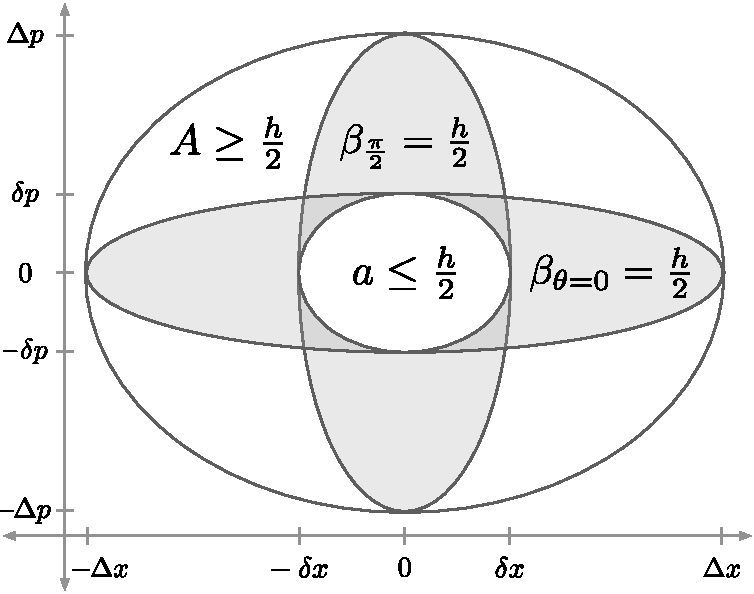
\includegraphics[width=\linewidth]{figures/principal_blobs.pdf}
\caption{\textbf{Capacity, quantum blobs at principal axes, and resolution.} The state's covariance ellipsoid has action capacity $A = \pi \, \Delta x \, \Delta p \ge h/2$. The quantum blob family (Fig.~\ref{fig:quantum_blobs}) has two members at the principal axes, $\beta_{\theta=0} = \pi \, \Delta x \, \delta p = h/2$ and $\beta_{\pi/2} = \pi \,\delta x \,\Delta p = h/2$. The resolution $a$ is an ellipse with semi-axes $\delta x, \delta p$ and action $a = \pi \, \delta x \, \delta p = \pi\hbar^2/(\Delta x\,\Delta p)$. $A$ circumscribes $\beta_{\theta=0}$ and $\beta_{\pi/2}$, which circumscribe $a$.}
\label{fig:principal_blobs}
\end{figure}

\begin{figure}[!htbp]
\centering
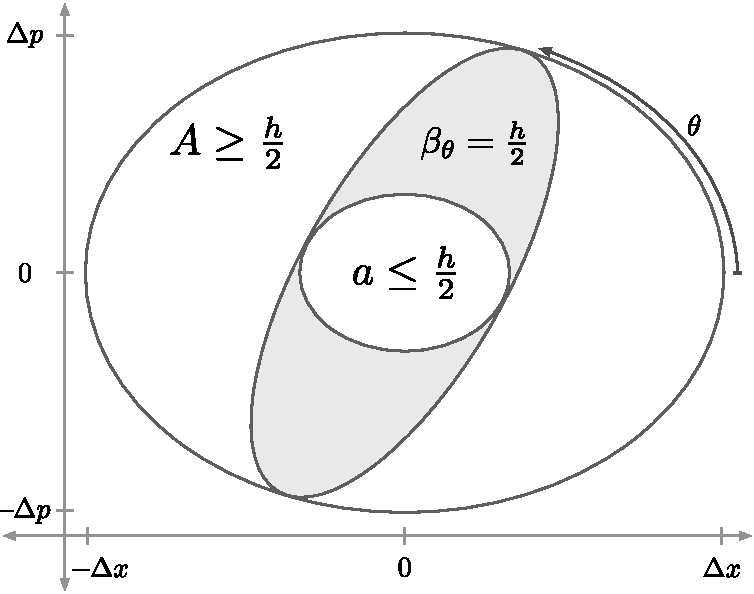
\includegraphics[width=\linewidth]{figures/quantum_blobs.pdf}
\caption{\textbf{Capacity, quantum blob family, and resolution.} Action capacity $A$ circumscribes the quantum blob family $\{\beta_\theta\}$, which circumscribes resolution $a$. Across $\theta$ the blob family deforms at constant action $\beta_\theta = h/2$. At the principal angles $\theta = 0$ and $\theta = \pi/2$, the family recovers $\beta_{\theta=0}$ and $\beta_{\pi/2}$ from Fig.~\ref{fig:principal_blobs}.}
\label{fig:quantum_blobs}
\end{figure}

\begin{figure*}[!tp]
\centering
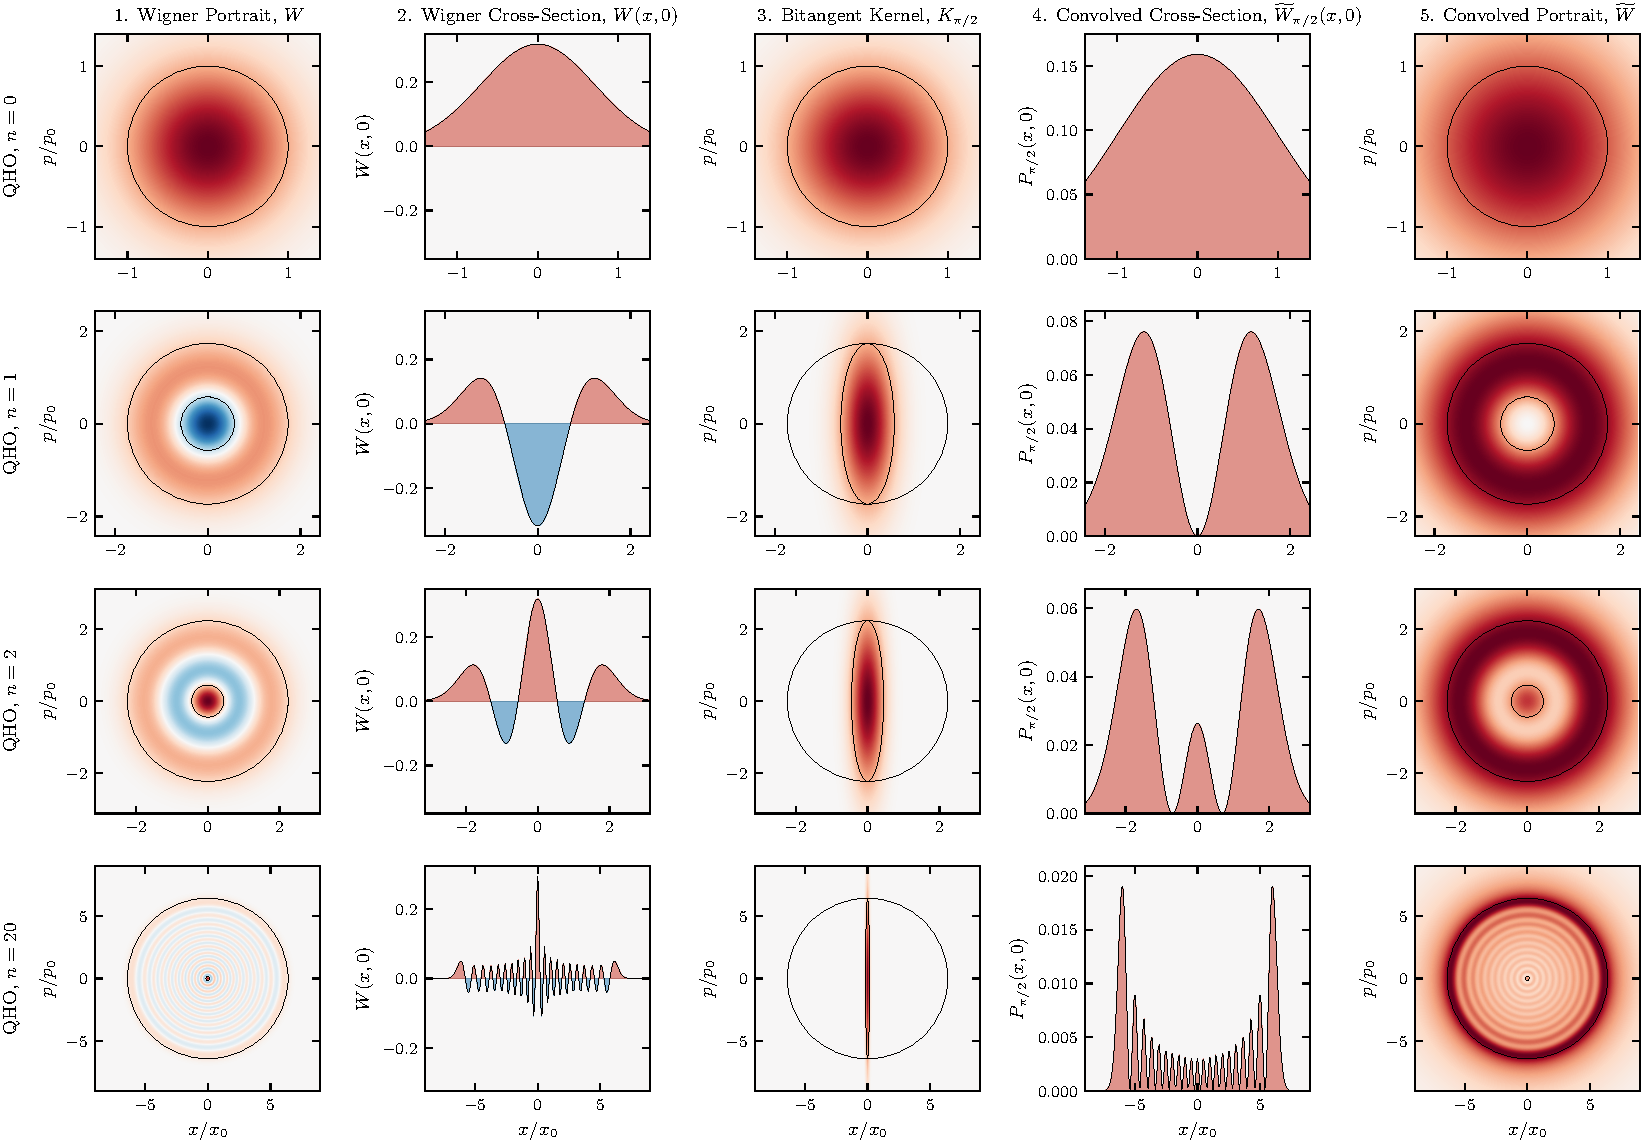
\includegraphics[width=\textwidth]{figures/harmonic.pdf}
\caption{\textbf{Harmonic oscillator.} Rows correspond to Fock states $n = 0, 1, 2, 20$ with action capacity $A/(h/2) = 2n+1$. Column 1: Wigner function $W(x, p)$ (negativity in blue) overlaid with the capacity $A$ and resolution $a$. Centered at the covariance origin, $a$ marks the resolution of the finest structure (the Zurek scale) of the bare, unconvolved Wigner function. Column 2: Cross-section $W(x, 0)$ exhibiting negative dips. Column 3: Quantum kernel $K_{\pi/2}$ overlaid with $A$ and the quantum blob $\beta_{\pi/2}$ (action $h/2$, restoring Planck's quantum of action). Column 4: Convolved cross-section $\widetilde W_{\pi/2}(x, 0)$ at quadrature angle $\theta = \pi/2$, which is non-negative. Column 5: The portrait $\widetilde W(x, p)$, integrated over the blob family across all $\theta$, overlaid with $A$ and $a$ (symplectic polar duals). It is everywhere non-negative, with positive lobes at the positions of those in $W$, resolved at $a$. For the vacuum ($n = 0$), $A$ and $a$ coincide as a Gaussian blob at $A = h/2$. As $n$ increases, $A$ grows and $a$ reciprocally shrinks ($a\,A = (h/2)^2$). At $n = 20$, the rings condense toward a classical energy trajectory, leaving $a$ as a fine central ellipse. Axes are in the oscillator scales $x_0 = \sqrt{\hbar/m\omega}$ and $p_0 = \sqrt{\hbar m\omega}$.}
\label{fig:harmonic}
\end{figure*}

\begin{figure*}[!tp]
\centering
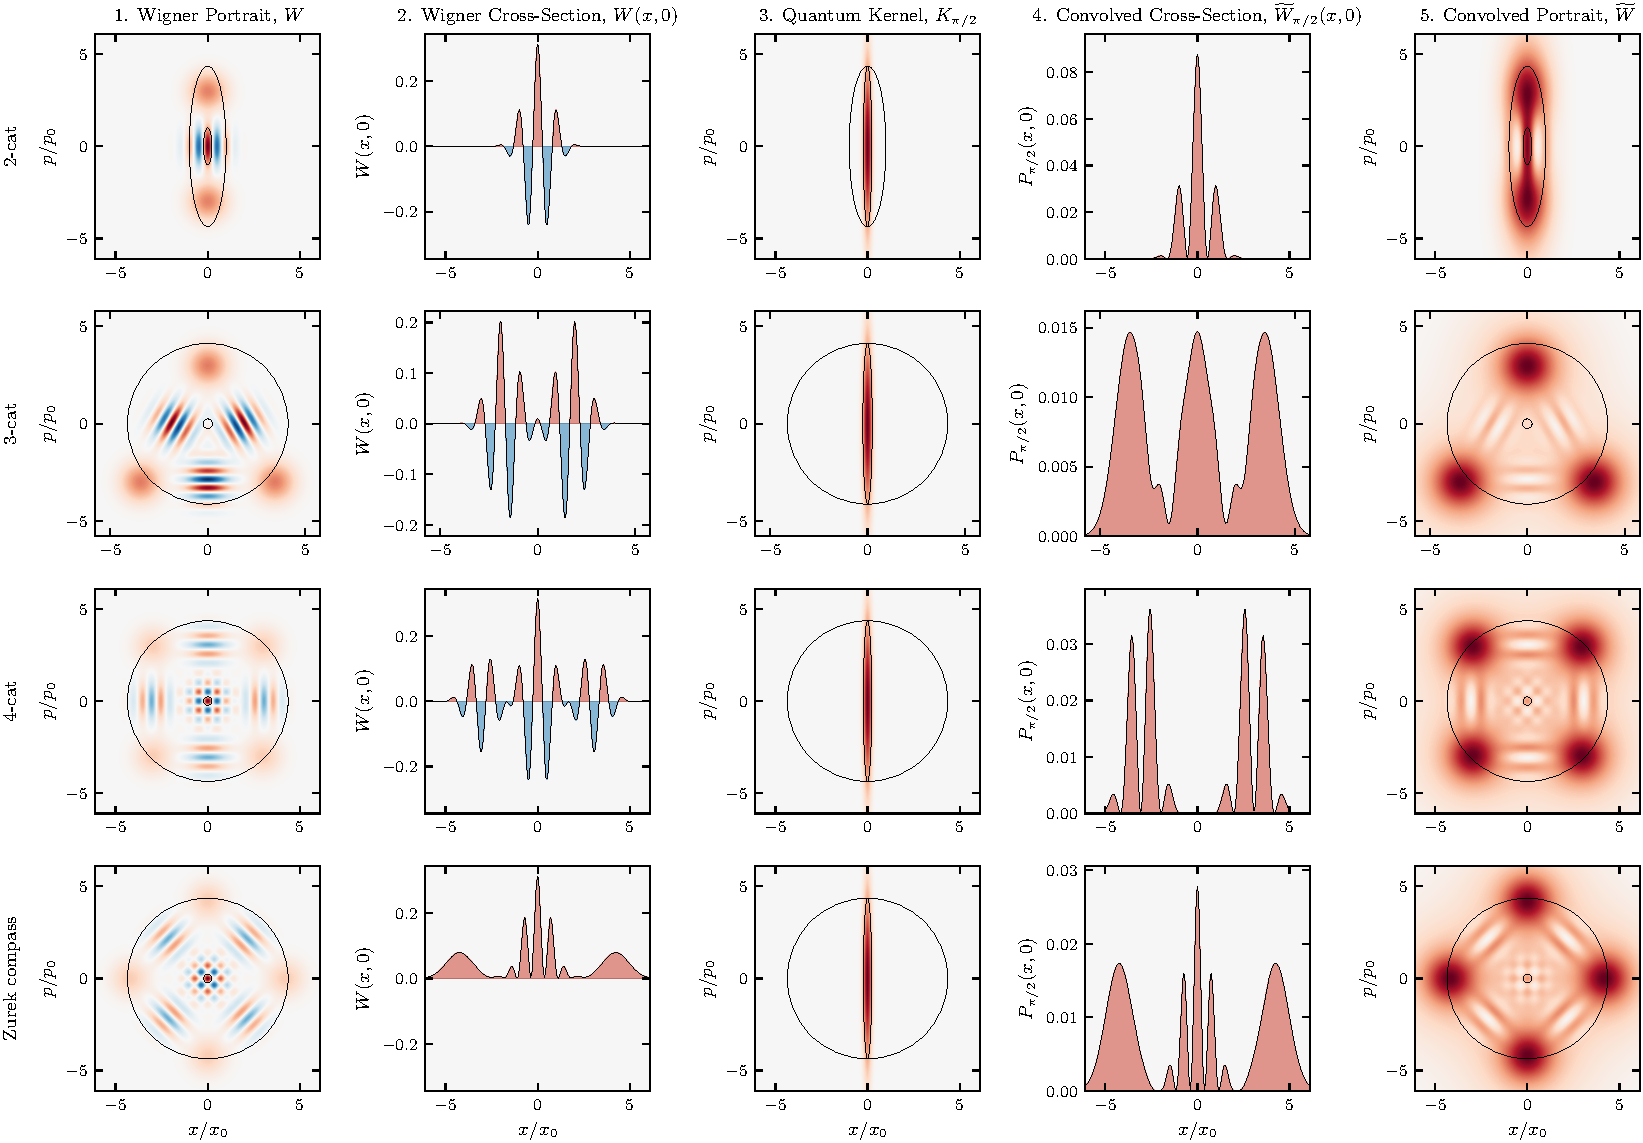
\includegraphics[width=\textwidth]{figures/cat.pdf}
\caption{\textbf{Cat states.} Rows correspond to the 2-cat, 3-cat, 4-cat, and Zurek compass states. Columns are as in Fig.~\ref{fig:harmonic}. As before, the portrait $\widetilde W$ (Column 5) is everywhere non-negative, with positive lobes at the positions of those in $W$, resolved at $a$. The 4-cat and Zurek compass states differ by a $\pi/4$ rotation in phase space.}
\label{fig:cat}
\end{figure*}

\begin{figure*}[!tp]
\centering
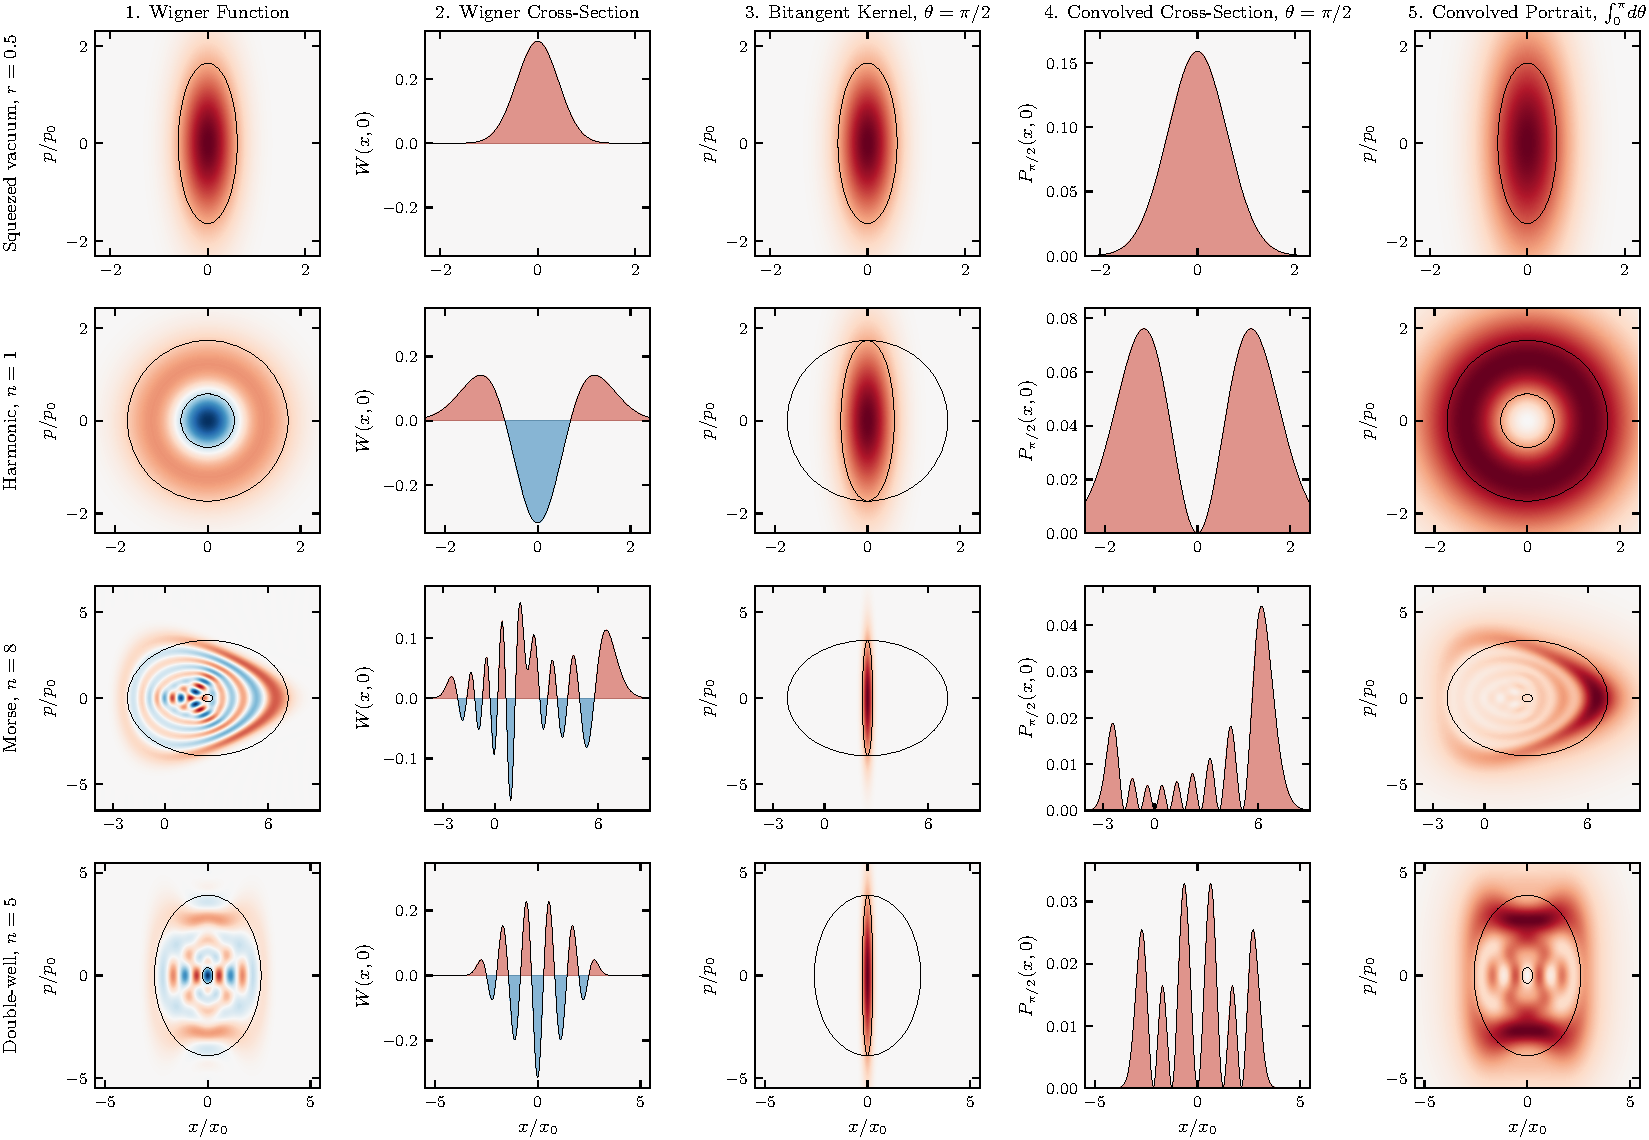
\includegraphics[width=\textwidth]{figures/eigen.pdf}
\caption{\textbf{Squeezed vacuum, eigenstates, and the Kerr crescent.} Rows correspond to the squeezed vacuum ($r = 0.5$), the Morse eigenstate ($n = 8$), the double-well eigenstate ($n = 5$), and the Kerr crescent, a coherent state sheared at constant photon number. Columns are as in Fig.~\ref{fig:harmonic}. The Kerr state is shown in the principal frame of its covariance, where the overlays are axis-aligned. The portrait $\widetilde W$ (Column 5) remains strictly non-negative across all four states, resolved at $a$.}
\label{fig:eigen}
\end{figure*}

% ===============================================================================
%  THE PHASE-SPACE GEOMETRY
% ===============================================================================
Planck divided phase space into elementary regions of action~\cite{planck1906}. Heisenberg's uncertainty principle $\sigma_x\,\sigma_p \ge \hbar/2$~\cite{kennard1927,robertson1929} fixes their minimum area but not their form, which a rotation of the axes redraws~\cite{schrodinger1930,cordero2018}. Geometrically, de Gosson replaced this coordinate-dependent tiling~\cite{degosson2003quantization} with one covariance ellipse per state~\cite{degossonluef2009irruption}, of semi-axes $\Delta x = \sqrt{2}\,\sigma_x$ and $\Delta p = \sqrt{2}\,\sigma_p$. This is the action capacity (Figs.~\ref{fig:principal_blobs},~\ref{fig:quantum_blobs}),
\begin{equation}
A = \pi\,\Delta x\,\Delta p \ge h/2.
\label{eq:action_capacity}
\end{equation}

% ===============================================================================
%  ZUREK SCALES AS A FAMILY OF DE GOSSON BLOBS
% ===============================================================================
The Wigner function carries structure at small scales. Zurek located those scales, $\delta p \sim \hbar/\Delta x$ and $\delta x \sim \hbar/\Delta p$, from the state's action capacity~\cite{zurek2001}. We identify them as the principal axes of a family of de Gosson quantum blobs~\cite{degosson2013qblobs} (Fig.~\ref{fig:principal_blobs}),
\begin{equation}
\beta_{\theta=0} = \pi\,\Delta x\,\delta p = h/2, \qquad \beta_{\pi/2} = \pi\,\delta x\,\Delta p = h/2.
\label{eq:principal_axis_blobs}
\end{equation}
The capacities $\Delta x, \Delta p$ run along the major axes, the resolutions $\delta x, \delta p$ along the minor.

Between these principal members the family $\{\beta_\theta\}$ deforms across $\theta \in [0,\pi)$ at constant action $h/2$ (Fig.~\ref{fig:quantum_blobs}). Capacity $A$ circumscribes each blob $\beta_\theta$. In the scaled coordinates $X = x/\Delta x$, $P = p/\Delta p$ every member is the same rigid ellipse rotated through $\theta$,
\begin{equation}
\beta_\theta = \left\{ (x,p) : X_\theta^{2} + \tfrac{A^2}{(\pi\hbar)^2}\, P_\theta^{2} \le 1 \right\},
\label{eq:atheta}
\end{equation}
inscribed in the unit disk. The quadratures $X_\theta = X\cos\theta + P\sin\theta$ and $P_\theta = -X\sin\theta + P\cos\theta$ are those of homodyne tomography at phase $\theta$.

% ===============================================================================
%  PER ANGLE NON-NEGATIVITY: THE QUANTUM KERNEL
% ===============================================================================
The Wigner function of the state is
\begin{equation}
W(x,p) = \frac{1}{\pi\hbar}\int \psi^*(x+s)\,\psi(x-s)\,e^{2ips/\hbar}\,ds.
\label{eq:wigner}
\end{equation}
The quantum kernel $K_\theta$ is a pure-state Wigner function, the centered Gaussian whose $h/2$ ellipse is the quantum blob $\beta_\theta$,
\begin{equation}
K_\theta(x, p) = \frac{1}{\pi\hbar}\exp\!\left[ -X_\theta^{2} - \tfrac{A^2}{(\pi\hbar)^2}\, P_\theta^{2} \right].
\label{eq:Ktheta}
\end{equation}
Convolving $W$ with $K_\theta$,
\begin{equation}
\widetilde W_\theta(x,p) = (W * K_\theta)(x,p),
\label{eq:Wtheta}
\end{equation}
lifts $W$ to Planck's quantum of action and renders $\widetilde W_\theta$ everywhere non-negative~\cite{cartwright1976,degosson2005bullsci,cordero2018}.

%===============================================================================
%  ALL-ANGLES RESOLUTION
%===============================================================================
Zurek also located the area scale $a_Z \sim \hbar \times (\hbar / A)$~\cite{zurek2001,zurek2003decoherence} of the chessboard structure in the compass state (Fig.~\ref{fig:cat}, column 1). We identify its coordinate-free form as the resolution $a$. It is the ellipse with semi-axes $\delta x, \delta p$ (Figs.~\ref{fig:principal_blobs},~\ref{fig:quantum_blobs}) and action
\begin{equation}
a = \pi\,\delta x\,\delta p = \frac{\pi\hbar^2}{\Delta x\,\Delta p}.
\label{eq:tildea}
\end{equation}
It is the resolution of the state's finest structure in the bare Wigner function (Figs.~\ref{fig:harmonic},~\ref{fig:eigen},~\ref{fig:cat},
column 1) and the symplectic polar dual of the capacity $A$~\cite{degosson2015indeterminacy}. The duality is reflexive, so $A$ and $a$ each fix the other, and antimonotone, so $a$ shrinks as $A$ grows~\cite{degosson2022polar}. The capacity $A$ circumscribes each blob $\beta_\theta$, which circumscribes the resolution $a$, each $\beta_\theta$ touching $a$ and $A$ twice, with $a \le \beta_\theta \le A$ (Fig.~\ref{fig:quantum_blobs}). Resolution and capacity are reciprocal at the quantum of action, $a\,A = (h/2)^2$.

% ===============================================================================
%  THE CONVOLVED PORTRAIT
% ===============================================================================

A single blob commits to a quadrature, a choice of coordinate the state does not favor. Integrating $\widetilde W_\theta$ over the family is coordinate-free, yielding the phase-space portrait,
\begin{equation}
\widetilde{W}(x,p) = \frac{1}{\pi}\int_0^\pi \widetilde W_\theta(x,p)\,d\theta.
\label{eq:tildeW}
\end{equation}
Each $\widetilde W_\theta \ge 0$, so $\widetilde W \ge 0$ everywhere. Where standard tomography inverts the marginals to recover the Wigner quasi-probability $W$~\cite{vogelrisken1989,lvovsky2009}, convolving $W$ with $\{K_\theta\}$ over the same $\theta$ builds the non-negative portrait $\widetilde W$.

The convolution and the integral are linear, so the family reduces to a single convolution,
\begin{equation}
\widetilde W = W * K, \qquad K = \frac{1}{\pi}\int_0^\pi K_\theta\,d\theta,
\label{eq:Kquorum}
\end{equation}
and the breadth of the kernel's Fourier transform $\widehat K$ sets the portrait's resolution. With $(\xi_x,\xi_p)$ the chord conjugate to $(x,p)$, integrating over $\theta$ bounds $\widehat K$ above by a single Gaussian,
\begin{equation}
\widehat{K}(\xi_x,\xi_p) \le \exp\!\left[ -\tfrac14\!\left( \delta x^{2}\,\xi_x^{2} + \delta p^{2}\,\xi_p^{2} \right) \right],
\label{eq:transfer}
\end{equation}
with equality at the origin. The bound cuts off at $\delta x$ and $\delta p$, so the portrait carries no structure finer than $\pi\,\delta x\,\delta p = a$, derived exactly in the Supplemental Material~\cite{zenododeposit}.

% ===============================================================================
%  UNIQUENESS OF BLOBS TO STATE
% ===============================================================================
A quantum blob $\beta_\theta$ too large for $A$ to circumscribe, or too
small to circumscribe $a$, is a blob of another state and
portrays that state, not this one~\cite{degosson2013qblobs,
degosson2022polar}. Every $h/2$ blob of this state is inscribed in $A$
and circumscribes $a$, touching each twice, so no $h/2$ smoothing of this
state resolves finer than $a$, and a kernel below $h/2$ fails to render
the portrait non-negative~\cite{cartwright1976,degosson2005bullsci}.
The finest resolution is $a$, reached by the family $\{\beta_\theta\}$
across $\theta \in [0,\pi)$.

%===============================================================================
%  GENERALIZATION
%===============================================================================
The principal frame, where $A$ is axis-aligned, costs no generality. The Wigner function transforms covariantly under the symplectic group~\cite{cordero2018}, so the map that diagonalizes a state's covariance carries it to this frame. The Kerr crescent, a sheared coherent state, is resolved this way (Fig.~\ref{fig:eigen}). In one degree of freedom, $A$ fixes the family uniquely, and the Zurek structure is already present for states with $A > h/2$. In higher dimensions, action $h/2$ no longer singles out a blob~\cite{degosson2013qblobs}, symplectic capacity and volume diverge, and the higher-dimensional case remains for future work.

%===============================================================================
%  DIFFERENTIATION
%===============================================================================
A fixed vacuum-width Gaussian~\cite{husimi1940} smooths every state equally, matching only the vacuum $A = h/2$ and erasing the detail of larger states $A > h/2$. Methods with a free parameter~\cite{wodkiewicz1984,appleby1998husimi,cahillglauber1969} resolve more finely, the scale set from outside the state. Here the state sets its own scale. Its action capacity $A$ fixes the resolution $a$ as the symplectic polar dual, with nothing left free.

%===============================================================================
%  NUMERICAL RESULTS
%===============================================================================
Figures~\ref{fig:harmonic},~\ref{fig:eigen}, and~\ref{fig:cat} show numerical results across twelve states. The portrait $\widetilde W$ is non-negative to machine precision, the chord-domain transfer carrying $W$ to $\widetilde W$ follows Eq.~\eqref{eq:transfer}, and the cross-spectral phase between $W$ and $\widetilde W$ vanishes. Across every state the portrait $\widetilde W$ resolves $W$ at $a$ and displaces nothing~\cite{zenododeposit}.

% ===============================================================================
%  DISCUSSION
% ===============================================================================
The uncertainty product $\sigma_x \sigma_p$ grows unbounded, the micro-to-macro transition Heisenberg~\cite{heisenberg1927} and Bohr~\cite{bohr1928} identified as requiring care. The quantum blob does not. As $A$ grows, the family $\{\beta_\theta\}$ deforms at fixed action $h/2$. Squeezing deforms a state by external apparatus~\cite{walls1983}. Here the scale called sub-Planck~\cite{zurek2001} is the minor axis $\delta$ of an $h/2$ blob, narrowing as the conjugate capacity $\Delta$ grows. A Schr\"odinger cat with capacity $\Delta p \sim 1$ kg$\cdot$m/s has resolution $\delta x = \hbar/\Delta p \sim 10^{-34}$ m, nineteen orders sub-nuclear~\cite{schrodinger1935trimmer}. The correspondence principle follows from $A \to \infty$ and $a \to 0$, the physical limit underlying the heuristic $h \to 0$. The resolution sharpens as the action capacity grows, $a = (h/2)^2 \,/ \,A$. We read this structure as the geometry of phase space itself, which de Gosson finds underlying the uncertainty principle~\cite{degossonluef2009irruption}.

% ===============================================================================
%  ACKNOWLEDGEMENTS
% ===============================================================================
\begin{acknowledgments}
The author thanks M. de Gosson for helpful comments. This research received no external funding. Computations used QuTiP~\cite{qutip5} and SciPy~\cite{scipy}. Code and Supplemental Material are openly available~\cite{zenododeposit}.
\end{acknowledgments}

\bibliography{main}

\end{document}